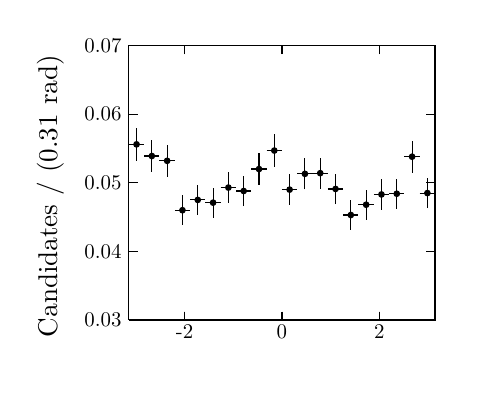
\begin{tikzpicture}
\pgfdeclareplotmark{cross} {
\pgfpathmoveto{\pgfpoint{-0.3\pgfplotmarksize}{\pgfplotmarksize}}
\pgfpathlineto{\pgfpoint{+0.3\pgfplotmarksize}{\pgfplotmarksize}}
\pgfpathlineto{\pgfpoint{+0.3\pgfplotmarksize}{0.3\pgfplotmarksize}}
\pgfpathlineto{\pgfpoint{+1\pgfplotmarksize}{0.3\pgfplotmarksize}}
\pgfpathlineto{\pgfpoint{+1\pgfplotmarksize}{-0.3\pgfplotmarksize}}
\pgfpathlineto{\pgfpoint{+0.3\pgfplotmarksize}{-0.3\pgfplotmarksize}}
\pgfpathlineto{\pgfpoint{+0.3\pgfplotmarksize}{-1.\pgfplotmarksize}}
\pgfpathlineto{\pgfpoint{-0.3\pgfplotmarksize}{-1.\pgfplotmarksize}}
\pgfpathlineto{\pgfpoint{-0.3\pgfplotmarksize}{-0.3\pgfplotmarksize}}
\pgfpathlineto{\pgfpoint{-1.\pgfplotmarksize}{-0.3\pgfplotmarksize}}
\pgfpathlineto{\pgfpoint{-1.\pgfplotmarksize}{0.3\pgfplotmarksize}}
\pgfpathlineto{\pgfpoint{-0.3\pgfplotmarksize}{0.3\pgfplotmarksize}}
\pgfpathclose
\pgfusepathqstroke
}
\pgfdeclareplotmark{cross*} {
\pgfpathmoveto{\pgfpoint{-0.3\pgfplotmarksize}{\pgfplotmarksize}}
\pgfpathlineto{\pgfpoint{+0.3\pgfplotmarksize}{\pgfplotmarksize}}
\pgfpathlineto{\pgfpoint{+0.3\pgfplotmarksize}{0.3\pgfplotmarksize}}
\pgfpathlineto{\pgfpoint{+1\pgfplotmarksize}{0.3\pgfplotmarksize}}
\pgfpathlineto{\pgfpoint{+1\pgfplotmarksize}{-0.3\pgfplotmarksize}}
\pgfpathlineto{\pgfpoint{+0.3\pgfplotmarksize}{-0.3\pgfplotmarksize}}
\pgfpathlineto{\pgfpoint{+0.3\pgfplotmarksize}{-1.\pgfplotmarksize}}
\pgfpathlineto{\pgfpoint{-0.3\pgfplotmarksize}{-1.\pgfplotmarksize}}
\pgfpathlineto{\pgfpoint{-0.3\pgfplotmarksize}{-0.3\pgfplotmarksize}}
\pgfpathlineto{\pgfpoint{-1.\pgfplotmarksize}{-0.3\pgfplotmarksize}}
\pgfpathlineto{\pgfpoint{-1.\pgfplotmarksize}{0.3\pgfplotmarksize}}
\pgfpathlineto{\pgfpoint{-0.3\pgfplotmarksize}{0.3\pgfplotmarksize}}
\pgfpathclose
\pgfusepathqfillstroke
}
\pgfdeclareplotmark{newstar} {
\pgfpathmoveto{\pgfqpoint{0pt}{\pgfplotmarksize}}
\pgfpathlineto{\pgfqpointpolar{44}{0.5\pgfplotmarksize}}
\pgfpathlineto{\pgfqpointpolar{18}{\pgfplotmarksize}}
\pgfpathlineto{\pgfqpointpolar{-20}{0.5\pgfplotmarksize}}
\pgfpathlineto{\pgfqpointpolar{-54}{\pgfplotmarksize}}
\pgfpathlineto{\pgfqpointpolar{-90}{0.5\pgfplotmarksize}}
\pgfpathlineto{\pgfqpointpolar{234}{\pgfplotmarksize}}
\pgfpathlineto{\pgfqpointpolar{198}{0.5\pgfplotmarksize}}
\pgfpathlineto{\pgfqpointpolar{162}{\pgfplotmarksize}}
\pgfpathlineto{\pgfqpointpolar{134}{0.5\pgfplotmarksize}}
\pgfpathclose
\pgfusepathqstroke
}
\pgfdeclareplotmark{newstar*} {
\pgfpathmoveto{\pgfqpoint{0pt}{\pgfplotmarksize}}
\pgfpathlineto{\pgfqpointpolar{44}{0.5\pgfplotmarksize}}
\pgfpathlineto{\pgfqpointpolar{18}{\pgfplotmarksize}}
\pgfpathlineto{\pgfqpointpolar{-20}{0.5\pgfplotmarksize}}
\pgfpathlineto{\pgfqpointpolar{-54}{\pgfplotmarksize}}
\pgfpathlineto{\pgfqpointpolar{-90}{0.5\pgfplotmarksize}}
\pgfpathlineto{\pgfqpointpolar{234}{\pgfplotmarksize}}
\pgfpathlineto{\pgfqpointpolar{198}{0.5\pgfplotmarksize}}
\pgfpathlineto{\pgfqpointpolar{162}{\pgfplotmarksize}}
\pgfpathlineto{\pgfqpointpolar{134}{0.5\pgfplotmarksize}}
\pgfpathclose
\pgfusepathqfillstroke
}
\definecolor{c}{rgb}{1,1,1};
\draw [color=c, fill=c] (5.1,4.68649) rectangle (9.9,9.0973);
\draw [color=c, fill=c] (5.772,5.39222) rectangle (9.66,8.87676);
\definecolor{c}{rgb}{0,0,0};
\draw [c] (5.772,5.39222) -- (5.772,8.87676) -- (9.66,8.87676) -- (9.66,5.39222) -- (5.772,5.39222);
\draw [c,line width=0.4] (5.8692,7.41691) -- (5.8692,7.62232);
\draw [c,line width=0.4] (5.8692,7.62232) -- (5.8692,7.82773);
\draw [c,line width=0.4] (5.772,7.62232) -- (5.8692,7.62232);
\draw [c,line width=0.4] (5.8692,7.62232) -- (5.9664,7.62232);
\foreach \P in {(5.8692,7.62232)}{\draw[mark options={color=c,fill=c},mark size=1.201201pt,mark=*,mark size=1pt] plot coordinates {\P};}
\draw [c,line width=0.4] (6.0636,7.27198) -- (6.0636,7.47423);
\draw [c,line width=0.4] (6.0636,7.47423) -- (6.0636,7.67648);
\draw [c,line width=0.4] (5.9664,7.47423) -- (6.0636,7.47423);
\draw [c,line width=0.4] (6.0636,7.47423) -- (6.1608,7.47423);
\foreach \P in {(6.0636,7.47423)}{\draw[mark options={color=c,fill=c},mark size=1.201201pt,mark=*,mark size=1pt] plot coordinates {\P};}
\draw [c,line width=0.4] (6.258,7.21232) -- (6.258,7.41325);
\draw [c,line width=0.4] (6.258,7.41325) -- (6.258,7.61418);
\draw [c,line width=0.4] (6.1608,7.41325) -- (6.258,7.41325);
\draw [c,line width=0.4] (6.258,7.41325) -- (6.3552,7.41325);
\foreach \P in {(6.258,7.41325)}{\draw[mark options={color=c,fill=c},mark size=1.201201pt,mark=*,mark size=1pt] plot coordinates {\P};}
\draw [c,line width=0.4] (6.4524,6.59919) -- (6.4524,6.78603);
\draw [c,line width=0.4] (6.4524,6.78603) -- (6.4524,6.97287);
\draw [c,line width=0.4] (6.3552,6.78603) -- (6.4524,6.78603);
\draw [c,line width=0.4] (6.4524,6.78603) -- (6.5496,6.78603);
\foreach \P in {(6.4524,6.78603)}{\draw[mark options={color=c,fill=c},mark size=1.201201pt,mark=*,mark size=1pt] plot coordinates {\P};}
\draw [c,line width=0.4] (6.6468,6.72684) -- (6.6468,6.9167);
\draw [c,line width=0.4] (6.6468,6.9167) -- (6.6468,7.10656);
\draw [c,line width=0.4] (6.5496,6.9167) -- (6.6468,6.9167);
\draw [c,line width=0.4] (6.6468,6.9167) -- (6.744,6.9167);
\foreach \P in {(6.6468,6.9167)}{\draw[mark options={color=c,fill=c},mark size=1.201201pt,mark=*,mark size=1pt] plot coordinates {\P};}
\draw [c,line width=0.4] (6.8412,6.6928) -- (6.8412,6.88186);
\draw [c,line width=0.4] (6.8412,6.88186) -- (6.8412,7.07092);
\draw [c,line width=0.4] (6.744,6.88186) -- (6.8412,6.88186);
\draw [c,line width=0.4] (6.8412,6.88186) -- (6.9384,6.88186);
\foreach \P in {(6.8412,6.88186)}{\draw[mark options={color=c,fill=c},mark size=1.201201pt,mark=*,mark size=1pt] plot coordinates {\P};}
\draw [c,line width=0.4] (7.0356,6.88008) -- (7.0356,7.07351);
\draw [c,line width=0.4] (7.0356,7.07351) -- (7.0356,7.26693);
\draw [c,line width=0.4] (6.9384,7.07351) -- (7.0356,7.07351);
\draw [c,line width=0.4] (7.0356,7.07351) -- (7.1328,7.07351);
\foreach \P in {(7.0356,7.07351)}{\draw[mark options={color=c,fill=c},mark size=1.201201pt,mark=*,mark size=1pt] plot coordinates {\P};}
\draw [c,line width=0.4] (7.23,6.83751) -- (7.23,7.02995);
\draw [c,line width=0.4] (7.23,7.02995) -- (7.23,7.22239);
\draw [c,line width=0.4] (7.1328,7.02995) -- (7.23,7.02995);
\draw [c,line width=0.4] (7.23,7.02995) -- (7.3272,7.02995);
\foreach \P in {(7.23,7.02995)}{\draw[mark options={color=c,fill=c},mark size=1.201201pt,mark=*,mark size=1pt] plot coordinates {\P};}
\draw [c,line width=0.4] (7.4244,7.11006) -- (7.4244,7.30871);
\draw [c,line width=0.4] (7.4244,7.30871) -- (7.4244,7.50736);
\draw [c,line width=0.4] (7.3272,7.30871) -- (7.4244,7.30871);
\draw [c,line width=0.4] (7.4244,7.30871) -- (7.5216,7.30871);
\foreach \P in {(7.4244,7.30871)}{\draw[mark options={color=c,fill=c},mark size=1.201201pt,mark=*,mark size=1pt] plot coordinates {\P};}
\draw [c,line width=0.4] (7.6188,7.34018) -- (7.6188,7.54392);
\draw [c,line width=0.4] (7.6188,7.54392) -- (7.6188,7.74766);
\draw [c,line width=0.4] (7.5216,7.54392) -- (7.6188,7.54392);
\draw [c,line width=0.4] (7.6188,7.54392) -- (7.716,7.54392);
\foreach \P in {(7.6188,7.54392)}{\draw[mark options={color=c,fill=c},mark size=1.201201pt,mark=*,mark size=1pt] plot coordinates {\P};}
\draw [c,line width=0.4] (7.8132,6.85454) -- (7.8132,7.04737);
\draw [c,line width=0.4] (7.8132,7.04737) -- (7.8132,7.24021);
\draw [c,line width=0.4] (7.716,7.04737) -- (7.8132,7.04737);
\draw [c,line width=0.4] (7.8132,7.04737) -- (7.9104,7.04737);
\foreach \P in {(7.8132,7.04737)}{\draw[mark options={color=c,fill=c},mark size=1.201201pt,mark=*,mark size=1pt] plot coordinates {\P};}
\draw [c,line width=0.4] (8.0076,7.05043) -- (8.0076,7.24773);
\draw [c,line width=0.4] (8.0076,7.24773) -- (8.0076,7.44504);
\draw [c,line width=0.4] (7.9104,7.24773) -- (8.0076,7.24773);
\draw [c,line width=0.4] (8.0076,7.24773) -- (8.1048,7.24773);
\foreach \P in {(8.0076,7.24773)}{\draw[mark options={color=c,fill=c},mark size=1.201201pt,mark=*,mark size=1pt] plot coordinates {\P};}
\draw [c,line width=0.4] (8.202,7.05895) -- (8.202,7.25644);
\draw [c,line width=0.4] (8.202,7.25644) -- (8.202,7.45395);
\draw [c,line width=0.4] (8.1048,7.25644) -- (8.202,7.25644);
\draw [c,line width=0.4] (8.202,7.25644) -- (8.2992,7.25644);
\foreach \P in {(8.202,7.25644)}{\draw[mark options={color=c,fill=c},mark size=1.201201pt,mark=*,mark size=1pt] plot coordinates {\P};}
\draw [c,line width=0.4] (8.3964,6.86305) -- (8.3964,7.05608);
\draw [c,line width=0.4] (8.3964,7.05608) -- (8.3964,7.24911);
\draw [c,line width=0.4] (8.2992,7.05608) -- (8.3964,7.05608);
\draw [c,line width=0.4] (8.3964,7.05608) -- (8.4936,7.05608);
\foreach \P in {(8.3964,7.05608)}{\draw[mark options={color=c,fill=c},mark size=1.201201pt,mark=*,mark size=1pt] plot coordinates {\P};}
\draw [c,line width=0.4] (8.5908,6.53964) -- (8.5908,6.72505);
\draw [c,line width=0.4] (8.5908,6.72505) -- (8.5908,6.91046);
\draw [c,line width=0.4] (8.4936,6.72505) -- (8.5908,6.72505);
\draw [c,line width=0.4] (8.5908,6.72505) -- (8.688,6.72505);
\foreach \P in {(8.5908,6.72505)}{\draw[mark options={color=c,fill=c},mark size=1.201201pt,mark=*,mark size=1pt] plot coordinates {\P};}
\draw [c,line width=0.4] (8.7852,6.66727) -- (8.7852,6.85572);
\draw [c,line width=0.4] (8.7852,6.85572) -- (8.7852,7.04418);
\draw [c,line width=0.4] (8.688,6.85572) -- (8.7852,6.85572);
\draw [c,line width=0.4] (8.7852,6.85572) -- (8.8824,6.85572);
\foreach \P in {(8.7852,6.85572)}{\draw[mark options={color=c,fill=c},mark size=1.201201pt,mark=*,mark size=1pt] plot coordinates {\P};}
\draw [c,line width=0.4] (8.9796,6.79494) -- (8.9796,6.98639);
\draw [c,line width=0.4] (8.9796,6.98639) -- (8.9796,7.17785);
\draw [c,line width=0.4] (8.8824,6.98639) -- (8.9796,6.98639);
\draw [c,line width=0.4] (8.9796,6.98639) -- (9.0768,6.98639);
\foreach \P in {(8.9796,6.98639)}{\draw[mark options={color=c,fill=c},mark size=1.201201pt,mark=*,mark size=1pt] plot coordinates {\P};}
\draw [c,line width=0.4] (9.174,6.80345) -- (9.174,6.9951);
\draw [c,line width=0.4] (9.174,6.9951) -- (9.174,7.18675);
\draw [c,line width=0.4] (9.0768,6.9951) -- (9.174,6.9951);
\draw [c,line width=0.4] (9.174,6.9951) -- (9.2712,6.9951);
\foreach \P in {(9.174,6.9951)}{\draw[mark options={color=c,fill=c},mark size=1.201201pt,mark=*,mark size=1pt] plot coordinates {\P};}
\draw [c,line width=0.4] (9.3684,7.26346) -- (9.3684,7.46552);
\draw [c,line width=0.4] (9.3684,7.46552) -- (9.3684,7.66758);
\draw [c,line width=0.4] (9.2712,7.46552) -- (9.3684,7.46552);
\draw [c,line width=0.4] (9.3684,7.46552) -- (9.4656,7.46552);
\foreach \P in {(9.3684,7.46552)}{\draw[mark options={color=c,fill=c},mark size=1.201201pt,mark=*,mark size=1pt] plot coordinates {\P};}
\draw [c,line width=0.4] (9.5628,6.81197) -- (9.5628,7.00382);
\draw [c,line width=0.4] (9.5628,7.00382) -- (9.5628,7.19566);
\draw [c,line width=0.4] (9.4656,7.00382) -- (9.5628,7.00382);
\draw [c,line width=0.4] (9.5628,7.00382) -- (9.66,7.00382);
\foreach \P in {(9.5628,7.00382)}{\draw[mark options={color=c,fill=c},mark size=1.201201pt,mark=*,mark size=1pt] plot coordinates {\P};}
\draw [c,line width=0.4] (5.772,5.39222) -- (9.66,5.39222);
\draw [anchor= east] (9.66,4.89821) node[scale=0.979628, rotate=0]{$\phihel$};
\draw [c,line width=0.4] (6.47841,5.4994) -- (6.47841,5.39222);
\draw [c,line width=0.4] (7.716,5.4994) -- (7.716,5.39222);
\draw [c,line width=0.4] (8.95359,5.4994) -- (8.95359,5.39222);
\draw [c,line width=0.4] (6.47841,5.4994) -- (6.47841,5.39222);
\draw [c,line width=0.4] (8.95359,5.4994) -- (8.95359,5.39222);
\draw [anchor=base] (6.47841,5.15403) node[scale=0.75356, rotate=0]{-2};
\draw [anchor=base] (7.716,5.15403) node[scale=0.75356, rotate=0]{0};
\draw [anchor=base] (8.95359,5.15403) node[scale=0.75356, rotate=0]{2};
\draw [c,line width=0.4] (5.772,8.87676) -- (9.66,8.87676);
\draw [c,line width=0.4] (6.47841,8.76957) -- (6.47841,8.87676);
\draw [c,line width=0.4] (7.716,8.76957) -- (7.716,8.87676);
\draw [c,line width=0.4] (8.95359,8.76957) -- (8.95359,8.87676);
\draw [c,line width=0.4] (6.47841,8.76957) -- (6.47841,8.87676);
\draw [c,line width=0.4] (8.95359,8.76957) -- (8.95359,8.87676);
\draw [c,line width=0.4] (5.772,5.39222) -- (5.772,8.87676);
\draw [anchor= east] (4.7736,8.87676) node[scale=0.979628, rotate=90]{Candidates / (0.31 rad)};
\draw [c,line width=0.4] (5.88576,5.39222) -- (5.772,5.39222);
\draw [c,line width=0.4] (5.88576,6.26335) -- (5.772,6.26335);
\draw [c,line width=0.4] (5.88576,7.13449) -- (5.772,7.13449);
\draw [c,line width=0.4] (5.88576,8.00562) -- (5.772,8.00562);
\draw [c,line width=0.4] (5.88576,8.87676) -- (5.772,8.87676);
\draw [anchor= east] (5.772,5.39222) node[scale=0.75356, rotate=0]{0.03};
\draw [anchor= east] (5.772,6.26335) node[scale=0.75356, rotate=0]{0.04};
\draw [anchor= east] (5.772,7.13449) node[scale=0.75356, rotate=0]{0.05};
\draw [anchor= east] (5.772,8.00562) node[scale=0.75356, rotate=0]{0.06};
\draw [anchor= east] (5.772,8.87676) node[scale=0.75356, rotate=0]{0.07};
\draw [c,line width=0.4] (9.66,5.39222) -- (9.66,8.87676);
\draw [c,line width=0.4] (9.54624,5.39222) -- (9.66,5.39222);
\draw [c,line width=0.4] (9.54624,6.26335) -- (9.66,6.26335);
\draw [c,line width=0.4] (9.54624,7.13449) -- (9.66,7.13449);
\draw [c,line width=0.4] (9.54624,8.00562) -- (9.66,8.00562);
\draw [c,line width=0.4] (9.54624,8.87676) -- (9.66,8.87676);
\end{tikzpicture}
